\documentclass{beamer}

\mode<presentation> {

%\usetheme{default}
%\usetheme{AnnArbor}
%\usetheme{Antibes}
%\usetheme{Bergen}
%\usetheme{Berkeley}
%\usetheme{Berlin}
%\usetheme{Boadilla}
%\usetheme{CambridgeUS}
%\usetheme{Copenhagen}
%\usetheme{Darmstadt}
%\usetheme{Dresden}
%\usetheme{Frankfurt}
%\usetheme{Goettingen}
%\usetheme{Hannover}
%\usetheme{Ilmenau}
%\usetheme{JuanLesPins}
%\usetheme{Luebeck}
\usetheme{Madrid}
%\usetheme{Malmoe}
%\usetheme{Marburg}
%\usetheme{Montpellier}
%\usetheme{PaloAlto}
%\usetheme{Pittsburgh}
%\usetheme{Rochester}
%\usetheme{Singapore}
%\usetheme{Szeged}
%\usetheme{Warsaw}


%\usecolortheme{albatross}
%\usecolortheme{beaver}
%\usecolortheme{beetle}
%\usecolortheme{crane}
%\usecolortheme{dolphin}
%\usecolortheme{dove}
%\usecolortheme{fly}
%\usecolortheme{lily}
%\usecolortheme{orchid}
%\usecolortheme{rose}
%\usecolortheme{seagull}
%\usecolortheme{seahorse}
%\usecolortheme{whale}
%\usecolortheme{wolverine}

%\setbeamertemplate{footline} % To remove the footer line in all slides uncomment this line
%\setbeamertemplate{footline}[page number] % To replace the footer line in all slides with a simple slide count uncomment this line

%\setbeamertemplate{navigation symbols}{} % To remove the navigation symbols from the bottom of all slides uncomment this line
}

\usepackage{graphicx} % Allows including images
\usepackage{booktabs} % Allows the use of \toprule, \midrule and \bottomrule in tables
\usepackage{amsfonts}
\usepackage{mathrsfs}
\usepackage{amsmath,amssymb,graphicx}

%----------------------------------------------------------------------------------------
%	TITLE PAGE
%----------------------------------------------------------------------------------------

\title["4.1"]{4.1: Probability Density Functions and Cumulative Distribution Functions}

\author{Taylor} 
\institute[UVA] 
{
University of Virginia \\
\medskip
\textit{} 
}
\date{} 

\begin{document}
%----------------------------------------------------------------------------------------

\begin{frame}
\titlepage 
\end{frame}
%----------------------------------------------------------------------------------------

\begin{frame}
\frametitle{Motivation}

In chapter 3, our discrete rvs had a finite or countably infinite number of possible values it could take on. Now we'll talk about continuous rvs. They can take on a whole interval/range of possible values. 

\end{frame}

%----------------------------------------------------------------------------------------

\begin{frame}
\frametitle{Definition}

Let $X$ be a continuous rv. 
\begin{definition}
The \textbf{probability density function} pdf of $X$ is the function $f(x)$ such that for any $a \le b$

\[
P(a \le X \le b) = \int_a^b f(x) dx
\]
\end{definition}

...it also has these properties
\begin{enumerate}
\item $f(x) \ge 0$ for all $x$
\item $\int_{-\infty}^{\infty}f(x) dx = 1$
\end{enumerate}

\end{frame}

%----------------------------------------------------------------------------------------
\begin{frame}
\frametitle{Definition}

\begin{definition}
The \textbf{cumulative distribution function (cdf)} for a cts rv $X$ is this function
\[
F(x) = \int_{-\infty}^x f(s) ds
\]
\end{definition}

\end{frame}

%----------------------------------------------------------------------------------------


\begin{frame}
\frametitle{Another fact}

If $X$ is continuous with pdf and cdf $f(x)$ and $F(x)$, respectively, then
\[
f(x) = \frac{d}{dx}F(x)
\]

(because of the fundamental theorem of calculus)
\end{frame}

%----------------------------------------------------------------------------------------

\begin{frame}
\frametitle{Definition}

Example of continous rv No. 1: the \textbf{uniform distribution} on the interval $[a,b]$:
\[
f(x) = f(x; a,b) = (b-a)^{-1}, \hspace{5mm} a \le x \le b
\]

\begin{center}
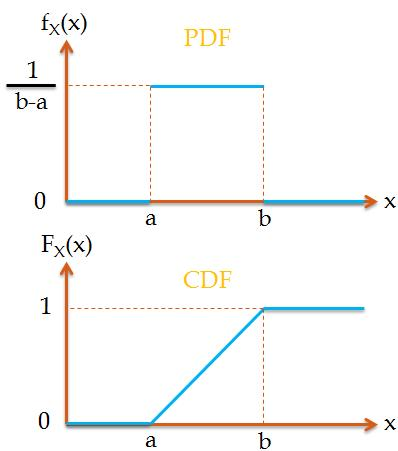
\includegraphics[width=50mm]{/home/taylor/UVa/all_teaching/3120_slides/4/4.1/pics/Continuous-Uniform_Distribution.jpg}
\end{center}

\end{frame}

%----------------------------------------------------------------------------------------

\begin{frame}
\frametitle{Derivation}

assuming $a \le x \le b$...
\begin{align*}
F(x) &= \int_{-\infty}^x f(s) ds \\
&= \int_{a}^x \frac{1}{b-a} ds \\
&= \frac{1}{b-a} (s)|_{s=a}^{s=x} \\
&= \frac{x-a}{b-a}
\end{align*}

\end{frame}
%----------------------------------------------------------------------------------------


\begin{frame}
\frametitle{Note}

Here is an important thing to remember about continuous rvs:

\[
P(X=c) = \int_c^c f(x) dx = \lim_{\epsilon \to 0} \int_{c - \epsilon}^{c+\epsilon} f(x) dx = 0
\]
so for any $a,b$

\[
P(a \le X \le b) = P(a < X < b) = P(a < X \le b) = P(a \le X < b)
\]
(we don't have to be careful about our inequalities like we do with discrete rvs...)
\end{frame}

%----------------------------------------------------------------------------------------


\begin{frame}
\frametitle{Another fact}

Let $X$ be a cts rv with pdf $f(x)$ and cdf $F(x)$. Then for any $a$
\[
P(X > a) = 1 - F_X(a)
\]
\[
P(a \le X \le b) = P(a < X \le b) = F_X(b) - F_X(a)
\]
\end{frame}

%----------------------------------------------------------------------------------------

\begin{frame}
\frametitle{Definition}

\begin{definition}
A \textbf{percentile} $\eta(p)$ associated with some percent $p$ of a cts rv $X$ is some number such that

\[
p = F[\eta(p)] = \int_{-\infty}^{\eta(p)} f(s)ds
\]
\end{definition}

i.e. it's some number such that $p$ \% of the data is behind it
\newline

Note: \textbf{quantiles} are just special cases of percentiles (e.g. quartiles = 25th,50th,75th percentiles) (e.g. deciles = 10th,20th,30th,40th,50th,60th,70th,80th,90th percentiles)
\newline

Note: the \textbf{median} is the 50th percentile
\end{frame}

%----------------------------------------------------------------------------------------

\begin{frame}
\frametitle{Definition}

\begin{definition}
A cts rv $X$ is \textbf{symmetric} if there is some point $c$ such that
\[
f(c-s) = f(c+s)
\]
for all $s$
\end{definition}

\end{frame}

%----------------------------------------------------------------------------------------



\begin{frame}
\frametitle{Example}

This is example 4.9 from page 167. We have the density $f(x) = \frac{3}{2}(1 - x^2)$ as long as $X \in [0,1]$. Find the 25\% percentile for this distribution.
\pause

\begin{align*}
\int_0^{\eta(.25)}\frac{3}{2}(1 - x^2)dx &= .25 \iff \\
\int_0^{\eta(.25)} \frac{3}{2} dx - \int_0^{\eta(.25)}\frac{3}{2}x^2 dx &= .25 \iff \\
\frac{3}{2} \eta - \frac{1}{2}\eta^3 = .25
\end{align*}


\end{frame}

%----------------------------------------------------------------------------------------



\begin{frame}
\frametitle{Example}

$X$ follows a \textbf{normal} or \textbf{gaussian distribution} if 

\[
f(x; \mu, \sigma^2)  = \frac{1}{ \sqrt{2 \pi \sigma^2} } \exp \left[ - \frac{(x - \mu)^2}{2 \sigma^2} \right]
\]

show that it is symmetric 
\pause

\begin{align*}
f(\mu - s) &= \frac{1}{ \sqrt{2 \pi \sigma^2} } \exp \left[ -\frac{(-s)^2}{2 \sigma^2} \right] \\
&= \frac{1}{ \sqrt{2 \pi \sigma^2} } \exp \left[ -\frac{(s)^2}{2 \sigma^2} \right] \\
&= f(\mu + s)
\end{align*}

and this holds for arbitrary $s$
\end{frame}

%----------------------------------------------------------------------------------------


\end{document} 